\documentclass[aspectratio=169,11pt]{beamer}

\usetheme{default}
\usefonttheme{professionalfonts}
\usepackage[T1]{fontenc}
\usepackage[default]{sourcesanspro}
\usepackage{amsmath,amssymb}
\usepackage{booktabs,tabularx,array,colortbl}
\usepackage{pgfplots}
\usepackage{appendixnumberbeamer}
\pgfplotsset{compat=1.17}

\definecolor{Ink}{HTML}{18212B}
\definecolor{Muted}{HTML}{5D6875}
\definecolor{Terra}{HTML}{9C3E2F}
\definecolor{Blue}{HTML}{2F6690}
\definecolor{Pale}{HTML}{EEF2F4}
\definecolor{Green}{HTML}{2C6E49}

\setbeamercolor{normal text}{fg=Ink,bg=white}
\setbeamercolor{frametitle}{fg=Ink,bg=white}
\setbeamercolor{alerted text}{fg=Terra}
\setbeamercolor{structure}{fg=Blue}
\setbeamercolor{footnote}{fg=Muted}
\setbeamercolor{footline}{fg=Muted,bg=white}
\setbeamertemplate{navigation symbols}{}
\setbeamertemplate{itemize item}{\raise0.15ex\hbox{\scriptsize\textbullet}}
\setbeamertemplate{itemize subitem}{\raise0.15ex\hbox{\scriptsize--}}
\setbeamerfont{frametitle}{size=\Large,series=\bfseries}
\setbeamerfont{title}{size=\huge,series=\bfseries}
\setbeamerfont{subtitle}{size=\large}
\setbeamerfont{footnote}{size=\tiny}
\setbeamertemplate{frametitle}{%
  \vspace{0.28em}\insertframetitle\par
  \vspace{0.12em}{\color{Terra}\rule{\textwidth}{0.8pt}}
}
\setbeamertemplate{footline}{%
  \leavevmode\hbox{\begin{beamercolorbox}[wd=\paperwidth,ht=2.5ex,dp=0.8ex,rightskip=1.2em]{footline}%
    \hfill\scriptsize\insertframenumber\,/\,\inserttotalframenumber
  \end{beamercolorbox}}
}

\newcommand{\source}[1]{\vfill{\color{Muted}\tiny Source: #1}}
\newcommand{\good}[1]{{\color{Green}\textbf{#1}}}
\newcommand{\bad}[1]{{\color{Terra}\textbf{#1}}}
\newcommand{\muted}[1]{{\color{Muted}#1}}
\newcommand{\tightitems}{\setlength{\itemsep}{0.55em}}
\newcolumntype{Y}{>{\raggedright\arraybackslash}X}

\title{The circulated calibration note}
\subtitle{What reproduces, what does not, and what M5 can currently support}
\author{Tommaso De Santo}
\date{Discussion with Corina \textbullet{} July 21, 2026}

\begin{document}

\begin{frame}[plain]
  \titlepage
\end{frame}

\begin{frame}{Audit result}
  \large
  The circulated parameter and moment tables reproduce the canonical M5 solution exactly.

  \vspace{1.0em}
  \begin{columns}[T,onlytextwidth]
    \column{0.30\textwidth}
      {\fontsize{29}{32}\selectfont\good{14 / 14}}\\[-0.1em]
      \textbf{parameter estimates}
    \column{0.30\textwidth}
      {\fontsize{29}{32}\selectfont\good{15 / 15}}\\[-0.1em]
      \textbf{model moments}
    \column{0.34\textwidth}
      {\fontsize{29}{32}\selectfont\bad{9 / 14}}\\[-0.1em]
      \textbf{effective rank at 1\%}
  \end{columns}

  \vspace{1.2em}
  The numerical result is reproducible. The structural interpretation is substantially less secure.
  \source{M5 strict repeated winner and local-identification audit.}
\end{frame}

\begin{frame}{Model architecture}
  \normalsize
  M5 links family needs to housing access and lifecycle balance sheets.

  \vspace{0.45em}
  \begin{columns}[T,onlytextwidth]
    \column{0.31\textwidth}
      \textbf{Family formation}
      \begin{itemize}\tightitems
        \item Completed family size chosen once
        \item One shared child-maturity clock
        \item No sequential birth hazards
      \end{itemize}
    \column{0.31\textwidth}
      \textbf{Housing and tenure}
      \begin{itemize}\tightitems
        \item Rent continuously up to 6 rooms
        \item Own one of $\{2,4,6,8,10\}$ rooms
        \item Purchase requires $(1-\phi)PH=0.2PH$
      \end{itemize}
    \column{0.31\textwidth}
      \textbf{Saving and bequests}
      \begin{itemize}\tightitems
        \item Liquid wealth may be negative
        \item Terminal estate is $b+PH$
        \item No amortizing mortgage contract
      \end{itemize}
  \end{columns}

  \vspace{0.2em}
  The model is appropriate for completed-fertility and housing-access mechanisms, not for birth timing or mortgage-contract claims.
  \source{Active M5 implementation and implementation ledger.}
\end{frame}

\begin{frame}{Calibration design}
  \begin{columns}[T,onlytextwidth]
    \column{0.47\textwidth}
      \large\textbf{Estimated jointly}
      \begin{itemize}\tightitems
        \item 14 preference, needs, tenure, supply, and bequest parameters
        \item 15 fertility, housing, ownership, wealth, and estate moments
        \item Weighted loss: $9.044$
      \end{itemize}
    \column{0.47\textwidth}
      \large\textbf{Maintained or external}
      \begin{itemize}\tightitems
        \item Four-year timing, $\sigma=2$, and housing-finance rates
        \item Income persistence and low innovation risk
        \item $\theta_n=0$ and one national housing market
      \end{itemize}
  \end{columns}

  \vspace{0.8em}
  \alert{The loss mixes inverse-variance and judgmental weights.} It ranks candidates under this target system; it is not a chi-squared statistic.
  \source{M5 parameter table, target-fit table, and objective definition.}
\end{frame}

\begin{frame}{Local identification}
  \begin{columns}[T,onlytextwidth]
    \column{0.28\textwidth}
      {\fontsize{34}{38}\selectfont\bad{9 / 14}}\\
      \large effective rank at $10^{-2}$
    \column{0.28\textwidth}
      {\fontsize{34}{38}\selectfont\bad{12 / 14}}\\
      \large effective rank at $10^{-3}$
    \column{0.34\textwidth}
      {\fontsize{34}{38}\selectfont\bad{2,926}}\\
      \large condition number
  \end{columns}

  \vspace{1.2em}
  The weakest direction jointly loads on
  \[
    (\bar h_0,\theta_1,\theta_0,\kappa_T).
  \]
  The moment-to-parameter discussion in the note is economic intuition, not evidence of one-to-one identification.
  \source{SMM-weighted Jacobian audit.}
\end{frame}

\begin{frame}{Loss decomposition}
  \begin{columns}[T,onlytextwidth]
    \column{0.64\textwidth}
      \resizebox{0.96\linewidth}{!}{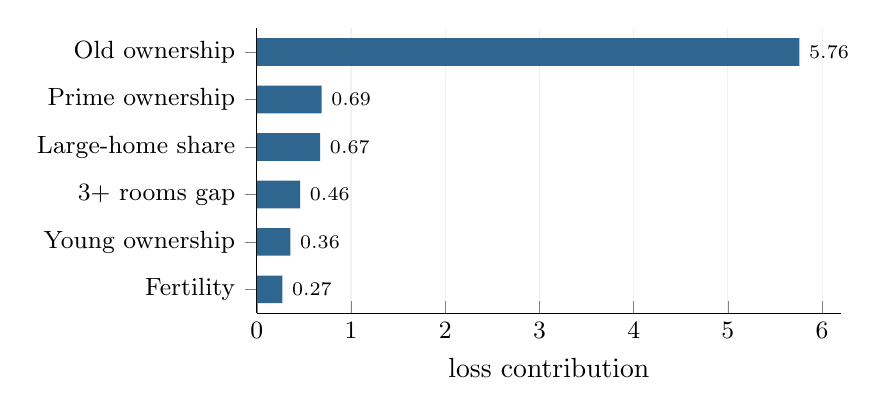
\begin{tikzpicture}
      \begin{axis}[
        xbar,
        width=9.0cm,height=5.2cm,
        xmin=0,xmax=6.2,
        y dir=reverse,
        symbolic y coords={Old ownership,Prime ownership,Large-home share,3+ rooms gap,Young ownership,Fertility},
        ytick=data,
        axis x line*=bottom,axis y line*=left,
        tick label style={font=\small},
        xlabel={loss contribution},
        xmajorgrids=true,grid style={Pale},
        nodes near coords,
        every node near coord/.append style={font=\scriptsize,anchor=west},
        enlarge y limits=0.10,
      ]
        \addplot[fill=Blue,draw=none] coordinates {
          (5.759,Old ownership)
          (0.687,Prime ownership)
          (0.673,Large-home share)
          (0.460,3+ rooms gap)
          (0.356,Young ownership)
          (0.271,Fertility)
        };
      \end{axis}
      \end{tikzpicture}}
    \column{0.32\textwidth}
      \vspace{2.0em}
      {\fontsize{29}{32}\selectfont\bad{63.7\%}}\\[0.25em]
      \large of total loss comes from ownership at ages 65--75.

      \vspace{1.5em}
      The estate median is close to its target; late-life tenure is not.
  \end{columns}
  \source{M5 target-fit table.}
\end{frame}

\begin{frame}{Late-life ownership}
  \begin{columns}[T,onlytextwidth]
    \column{0.66\textwidth}
      
\begin{tikzpicture}
      \begin{axis}[
        width=\linewidth,height=0.60\textheight,
        xmin=61,xmax=83,ymin=0.65,ymax=1.00,
        xtick={62,66,70,74,78,82},
        ytick={0.65,0.70,0.75,0.80,0.85,0.90,0.95,1.00},
        yticklabel style={/pgf/number format/.cd,fixed,precision=0},
        yticklabels={65\%,70\%,75\%,80\%,85\%,90\%,95\%,100\%},
        grid=major,grid style={Pale},
        legend style={draw=none,at={(0.5,-0.19)},anchor=north,legend columns=2},
        tick label style={font=\small},
      ]
        \addplot[Terra,very thick,mark=*] coordinates {(62,.9462)(66,.9521)(70,.9549)(74,.9552)(78,.9505)(82,.9084)};
        \addlegendentry{M5}
        \addplot[Blue,very thick,mark=*] coordinates {(62,.7442)(66,.7592)(70,.7699)(74,.7759)(78,.7605)(82,.7481)};
        \addlegendentry{ACS}
      \end{axis}
      \end{tikzpicture}
    \column{0.30\textwidth}
      \vspace{1.4em}
      {\fontsize{29}{32}\selectfont\bad{95.4\%}}\\
      \large M5, ages 65--75

      \vspace{1.2em}
      {\fontsize{29}{32}\selectfont\good{76.4\%}}\\
      \large ACS target

      \vspace{1.2em}
      Liquid wealth turns negative while ownership remains above 90\%.
  \end{columns}
  \source{M5 lifecycle diagnostics and ACS ownership profile.}
\end{frame}

\begin{frame}{Fit by empirical margin}
  \begin{columns}[T,onlytextwidth]
    \column{0.47\textwidth}
      \large\good{Close to target}
      \begin{itemize}\tightitems
        \item Completed childlessness
        \item First-child housing response
        \item Median estate and older nonhousing wealth
        \item Aggregate occupied rooms
      \end{itemize}
    \column{0.47\textwidth}
      \large\bad{Binding misses}
      \begin{itemize}\tightitems
        \item Old ownership: $+15.1$ bootstrap SE
        \item Large-home share: $+9.4$ SE
        \item Family ownership gap: $+8.0$ SE
        \item Prime ownership: $+4.1$ SE
        \item Young ownership: $-3.7$ SE
      \end{itemize}
  \end{columns}

  \vspace{0.7em}
  The bootstrap ratios are descriptive, not a joint specification test, because the active objective does not use the full covariance matrix.
  \source{M5 fit and July 6 bootstrap standard-error audit.}
\end{frame}

\begin{frame}{Target provenance}
  \large
  Two headline targets are not presently reproducible from a repository builder:
  \[
    \text{completed fertility}=1.918,
    \qquad
    \text{childlessness}=0.188.
  \]

  The note says CPS, but the year, age window, children-ever-born variable, and weights are not pinned down.

  \vspace{0.7em}
  If both targets were removed without replacement, the calibration would have only 13 verified moments for 14 free parameters.

  \alert{They must be sourced, replaced by equally informative moments, or paired with an external restriction.}
  \source{July 6 target-reproduction audit.}
\end{frame}

\begin{frame}{Evidence after circulation}
  \begin{columns}[T,onlytextwidth]
    \column{0.31\textwidth}
      \textbf{Income frontier}
      \begin{itemize}\tightitems
        \item The M5 bundle is infeasible already at $\sigma_z=0.09$
        \item Lowering $\bar c_0$, not a small transfer floor, moves the frontier
      \end{itemize}
    \column{0.31\textwidth}
      \textbf{Transfer-floor probe}
      \begin{itemize}\tightitems
        \item Honest risk raises the estate tail
        \item Young wealth rises to $1.33$, far above the $0.18$ target
      \end{itemize}
    \column{0.31\textwidth}
      \textbf{E1 experiment}
      \begin{itemize}\tightitems
        \item Repairs late-life ownership and the estate tail
        \item Worsens fertility and first-child housing fit
        \item Loss rises from $9.04$ to $12.61$
      \end{itemize}
  \end{columns}

  \vspace{0.8em}
  These exercises clarify the trade-offs; none is a replacement baseline.
  \source{July 18 frontier and floor probes; July 19 E1 collection report.}
\end{frame}

\begin{frame}{Defensible interpretation}
  \large
  M5 is a reproducible, provisional calibration for studying how family housing needs interact with tenure and down-payment access.

  \vspace{0.9em}
  It does \textbf{not} currently support:
  \begin{itemize}\tightitems
    \item precise estimates of all 14 structural parameters;
    \item claims about sequential birth timing or mortgage contracts;
    \item a well-identified late-life portfolio or housing-exit mechanism;
    \item formal specification testing based on the scalar loss.
  \end{itemize}

  \vspace{0.5em}
  The next baseline should be judged by whether it preserves the housing-fertility mechanism while repairing provenance, identification, and late-life behavior.
\end{frame}

\begin{frame}{Questions for the next baseline}
  \large
  \begin{enumerate}
    \setlength{\itemsep}{1.05em}
    \item Is one-shot completed fertility acceptable if timing claims are removed?
    \item Should the next baseline prioritize income insurance or late-life housing exit?
    \item Should weak bequest and tenure parameters be externally fixed or newly identified?
    \item Which paper claims actually require a credible late-life portfolio block?
  \end{enumerate}
\end{frame}

\appendix

\begin{frame}{M5 parameter estimates}
\scriptsize
\centering
\begin{tabular}{lrrl@{\qquad}lrrl}
\toprule
Parameter & Estimate & Bounds & Status & Parameter & Estimate & Bounds & Status\\
\midrule
$\beta_{ann}$ & .9912 & [.800,.9995] & est. & $\psi_{child}$ & .1979 & [-3,3] & est.\\
$\alpha_c$ & .5912 & [.02,.98] & est. & $\kappa_F$ & 2.0434 & [.02,50] & est.\\
$\bar c_0$ & 1.2596 & [0,2] & est. & $\chi_O$ & 1.1133 & [.1,5] & est.\\
$\bar c_n$ & .3929 & [0,3] & est. & $\bar H$ & 8.6456 & [.2,80] & est.\\
$\bar h_0$ & .3915 & [.05,5.8] & est. & $\theta_0$ & .3118 & [0,8] & est.\\
$\bar h_{jump}$ & 1.6021 & [0,8] & est. & $\theta_1$ & .3973 & [.02,16] & est.\\
$\bar h_n$ & .1644 & [0,5] & est. & $\kappa_T$ & .0100 & [0,.12] & est.\\
&&&& $\theta_n$ & 0 & external & fixed\\
\bottomrule
\end{tabular}

\vspace{0.8em}
No estimate is mechanically near its search bound. That does not imply precise identification.
\source{M5 parameter collector.}
\end{frame}

\begin{frame}{Target fit: fertility, housing, and young wealth}
\tiny
\centering
\begin{tabularx}{\textwidth}{Yrrrrr}
\toprule
Moment & Data & Model & Gap & Weight & Loss\\
\midrule
Completed-fertility-equivalent$^{*}$ & 1.918 & 2.034 & .116 & 20.0 & .271\\
Completed childlessness$^{*}$ & .188 & .189 & .001 & 20.0 & .000\\
Ownership, ages 30--55 & .575 & .658 & .083 & 100.0 & .687\\
New-parent ownership gap & .168 & .219 & .052 & 45.0 & .121\\
First-child rooms response & .664 & .681 & .016 & 14.0 & .004\\
Childless-renter mean rooms & 3.805 & 3.963 & .158 & 6.0 & .150\\
Childless-owner share, 6+ rooms & .596 & .760 & .164 & 25.0 & .673\\
Young liquid wealth / income & .179 & .328 & .149 & 12.0 & .265\\
\bottomrule
\end{tabularx}

\vspace{0.6em}
\raggedright $^{*}$Source-unconfirmed in the repository reproduction audit.
\end{frame}

\begin{frame}{Target fit: tenure, estates, and aggregates}
\tiny
\centering
\begin{tabularx}{\textwidth}{Yrrrrr}
\toprule
Moment & Data & Model & Gap & Weight & Loss\\
\midrule
Owner-renter rooms gap & 2.419 & 2.323 & -.096 & 12.0 & .111\\
Ownership, ages 25--34 & .341 & .274 & -.067 & 80.0 & .356\\
Rooms gap, 3+ versus 1--2 children & .368 & .607 & .240 & 8.0 & .460\\
Median estate / income & 6.501 & 6.431 & -.070 & 18.6 & .092\\
Nonhousing wealth $\geq$ income & .608 & .610 & .002 & 9435.2 & .027\\
\rowcolor{Terra!10} Ownership, ages 65--75 & .764 & .954 & .190 & 160.0 & \textbf{5.759}\\
Mean occupied rooms & 5.780 & 5.673 & -.107 & 6.0 & .069\\
\midrule
\textbf{Total} &&&&& \textbf{9.044}\\
\bottomrule
\end{tabularx}
\end{frame}

\begin{frame}{Source qualifications}
\small
\begin{itemize}\tightitems
  \item The PDF circulated on July 17 reports a two-plus-versus-one-child estate gap of $0.101$. The later source adds that it is statistically insignificant (bootstrap SE $0.563$).
  \item The later source also notes that PSID nonhousing wealth includes business wealth, retirement accounts, and other assets absent from M5.
  \item External values were checked against the 2023 SSA life table, Greaney, Parkhomenko, and Van Nieuwerburgh (2025), and Saiz (2010).
\end{itemize}

\vspace{0.8em}
The circulated PDF, not the subsequently edited TeX file, is the record of what recipients saw.
\end{frame}

\end{document}
